\chapter{Implementation}
\label{cha:implementation}

\begin{figure}
  \centering
  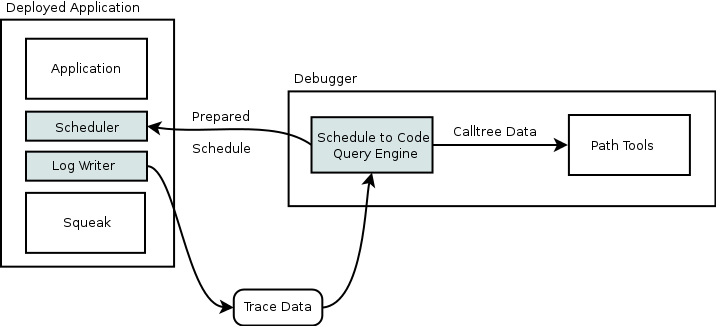
\includegraphics[width=0.9\linewidth]{structure}
  \caption{Interactions in the Prototype}
  \label{fig:structure}
\end{figure}

We evaluated our approach in a prototype for distributed applications
using \ac{http} to communicate, implemented in
Squeak/Smalltalk~\cite{Ingalls1997}. In this chapter, we explain how
we hooked into the entry and exit points for network communication,
for which we used \emph{ContextS}~\cite{Hirschfeld2008}, an
implementation of \ac{cop} for Squeak/Smalltalk. We already mentioned
that we built on earlier work about online analysis of runtime
behavior, implemented in the \emph{Path Tools} suite, and we have
based our debugging tool and visualization on the Path Tools
suite. \autoref{fig:structure} shows how our protoypes' components
interact. Applications are instrumented with ContextS to include a
logging and a scheduler layer. The logging creates trace data that is
used by our query engine to display the network communication patterns
with the Path Tools and provide any recorded call tree data. When the
developer chooses a schedule for re-execution, queries are attached to
the schedule events, the prepared schedule is sent to the scheduler,
and the application is re-executed. The scheduler shapes the
communication during re-execution to match the schedule and records
any additional information using the same mechanism as the log
writer. The resulting trace data is again sent to the query engine,
which passes the newly recorded information to the Path Tools for the
developer to inspect.

\section{Tracing Communication Patterns}
\label{sec:trac-comm-patt}

One way to implement the logging of logical communication schedules is
tracing the appropriate code executions in the system. For our
application, we identified the methods in a Squeak image where
\ac{http} requests are received and responses are generated. Our
example application used, besides the standard library \ac{http}
communication, the \emph{KomHttpServer} for receiving requests.

Tracing communication at different levels of granularity was vital to
verify our approach in a prototype. We chose ContextS so we could
easily add various layers with different logging mechanics for
experimentation. Additionally, ContextS layers are easy to manage in
Monticello, the \ac{vcs} of Squeak. This allowed us to keep the
tracing implementation as a separate project an thus fairly
independent of the traced system.

The combined log includes all events that were recorded between two
particular points in time. These points in time are given by the start
and finish of our diagnosis to reproduce a failure. Re-executing such
a diagnosis a number of times yields different time slices of
communication. We present these logs in a diagram with events as data
points and logical time on the x-axis. Because events are data points,
and there may be many events in one schedule, our visualization scales
all events to fit into one window. For many events, this allows
developers to get a high-level overview of the activity throughout the
system without swamping with detail. In \autoref{fig:comm-overview} we
see such an overview. While we cannot make out details, we can see
that the service running on \emph{localhost} port 5001 is active more
consistently than the one below it, running on port 5002. This
high-level pattern communication pattern may already provide some
insight as to how the system works.

\begin{figure}
  \centering
  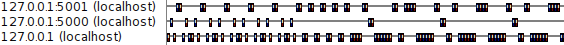
\includegraphics[width=0.95\linewidth]{comm-overview}
  \caption{Communication Schedule Overview}
  \label{fig:comm-overview}
\end{figure}

\autoref{fig:comm-logs} shows an example of a very small communication
schedule. We show the number of diagnosis runs that yielded this
particular schedule (\textcircled{1}), and how many events there are
in this schedule. The color of the box shows whether there were any
errors, such as failed assertions, during the diagnosis' execution by
turning from green to yellow. The recorded communicating servers
(\textcircled{2}) are presented as \textsc{IP} address labels on the
y-axis, with the associated port (if any). If that address resolves to
a host name, it is added in brackets. \emph{Lifelines} extend from the
endpoints, so events on the right-hand side can be easily associated
to a particular server. Each box represents an event with outgoing
events (\textcircled{3}) in red and incoming events (\textcircled{4})
in blue. The boxes in this visualization represent a point in time
rather than a time span, and their width is simply as wide as possible
to still show all events within the graph. Because each box shows the
first few bytes of captured message data if such has been captured, it
is useful to have boxes as wide as possible.

\begin{figure}
  \centering
  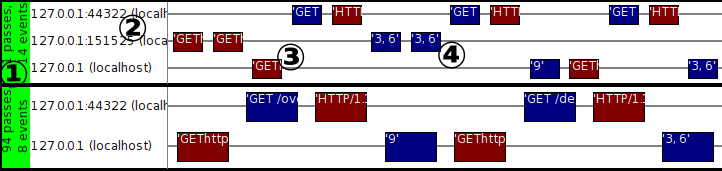
\includegraphics[width=\linewidth]{comm-log}
  \caption{Captured Communication Logs}
  \label{fig:comm-logs}
\end{figure}

\subsection{Distributed Context-oriented Computing}
\label{sec:distr-cont-orient}

ContextS layers can be dynamically enabled and disabled to extend
methods at runtime. For a distributed system, these layer activations
have to be distributed across the network, so enabling a particular
tracing mechanism on one system carries over to another. This can be
achieved in various ways. Because our layers are implemented for
\ac{http} requests only, we decided to propagate layers in a custom
\ac{http} header, \texttt{X-DCOPActiveLayers}, an application specific
header in accordance with RFC 2047. This header contains not the names
of the currently active layers, but, as suggested in~\cite{Rho2011},
an ontology describing those layers. This decouples the layer names on
our particular implementation from possible other implementations and
their layer names, by describing what layers do instead. Those headers
will be ignored by conforming implementations that do not use our
tracing package. On systems that do use our tracing, we read the list
and activate the layers globally as required.

Most Web application frameworks employ the \emph{inversion-of-control
  principle}, which does not work well for ContextS. In ContextS,
layer activations are valid for the dynamic scope of the execution,
and do not propagate upwards the stack from the point of
activation. This problem with \ac{cop} in the context of
inversion-of-control frameworks is known and has been treated in
recent work~\cite{Appeltauer2012,Appeltauer2012Phd}. We have not
implemented the mechanism to deal with this problem, so our prototype
is not able to activate layers across the network. Rather, the
required layers are simply active all of the time.

In related work, DejaVu uses a similar mechanism on the transport
layer that involves embedding and, on the remote end, stripping magic
bytes in \ac{tcp} packages~\cite{Konuru2000} to propagate
meta-information for tracing.

\subsection{Tracer Entry Points}
\label{sec:tracer-entry-points}

Tracing \ac{http} requests with ContextS entails finding and layering
methods in frameworks and standard library that create and receive
\ac{http} requests. In our example, using the Squeak standard library
and the KomHttpServer framework, this included layering only 3
methods.

Extending the implementation to work for other Squeak Web servers or
other application layer frameworks such as relational database
adapters is trivially possible. The actually captured data only
includes the local logical timestamp, as well as the sender and
receiver of the message.

\subsection{Trace Format}
\label{sec:trace-format}

To actually implement our approach for different runtimes and debug
across languages, an interchangeable trace format is necessary. We
have not implemented such a format. Our prototype is Squeak-based, so
the interchange format consists of a Squeak store string, which can be
recompiled into a collection of trace events. Each trace event, here,
is an object with a logical timestamp, receiver and sender \textsc{IP}
and port.

An interchangeable trace format is trivial to implement, however. To
exchange logs, we only need a way to transfer collections of event
3-tuples that include strings and integers which almost any
data-interchange format should be able to. \ac{json} seems to be a
natural choice, both because it is widely used and parsers are readily
available for a variety of languages, and because it is the most
common format in Web development.

\section{Communication Diffing}
\label{sec:diff-comm}

As per our design (\cf{\autoref{sec:comm-constr-analys}}), we regard
each communication schedule as a sequence diagram with only
asynchronous message sends. To help developers find differences in the
schedule, we want to automatically differentiate traces to show areas
of high and low variance in the schedule. For $N$ servers, at any one
logical time, there are at most $N$ network events. Comparing
different communication schedules can thus be done by comparing each
logical time in order, similar to how a patch algorithm compares files
at different versions.

\subsection{Difference Format and Visualization}
\label{sec:diff-form-visu}

The choice of algorithm for automatic differentiation can have a huge
impact on the usefulness of the result. There are various algorithms
to differentiate tree structures~\cite{Bischof2008AiA}. We treat our
communication schedules as call trees with only asynchronous
communication. That means they can be transformed into a linear form,
which makes them suited for the linear differential algorithms used
for file comparison. Of those, we chose the \ac{lcs} algorithm to
create differential schedules.

We can assume that schedules will vary in some events or
event-sequences, but will be equivalent for some length around those
variances. \ac{lcs} dynamically finds the longest matching
sub-sequence between two pieces of data. For comparing two schedules,
we choose one as the \emph{base} and the other as the change. In
\autoref{fig:comm-diff} we show such a differential schedule between
the base at the top and the comparison schedule at the bottom.

The differences between the schedules are marked in red. If we compare
the overall number of events, we can see that both the base schedule
at the stop and the comparison schedule at the bottom have the same
number of events. They are equivalent up to the first red marker,
where the comparison schedule sends out a \texttt{GET} request that
does not occur in the base schedule. If we follow the differential,
however, we can see that the schedules are equivalent again for four
more events until the second red marker. At that point, a \texttt{GET}
request sent in the base schedule does not occur in the comparison
schedule. Afterward, both are equivalent up to the end.

\begin{figure}
  \centering
  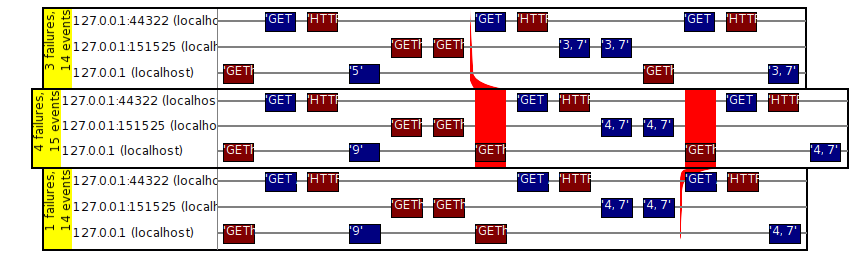
\includegraphics[width=\linewidth]{comm-diff}
  \caption{A Simple Differential Between 2 Schedules}
  \label{fig:comm-diff}
\end{figure}

\subsection{Correlating Variances and Failures}
\label{sec:corr-vari-fail}

Not all variances will usually contribute to the failure, yet, for
large numbers of runs we may have more variances than common
sub-sequences. Simple red/white differentials are not very helpful in
this case, as they do not significantly reduce the search space to aid
developers in their search for the problem. Due to this, we weigh
variances according to a number of rules, which have been in described
in \autoref{sec:assoc-vari-with}.

The heuristic probability distribution is mapped onto hue values from
zero to sixty degrees, which corresponds to full red and full yellow,
respectively. For variances that the heuristic recognizes to have no
impact on the failure, we assign the color gray.

To review variances between passing runs, we assign hue values
depending on the amount of variance on each particular network
event. The function \emph{hue}, below, shows how we map the each event
onto a range from 0 to 1. We then map this range onto a range from 0
to 60, corresponding to the colors from red to yellow in the
\textsc{hsl} color space. We assign alpha values from 0 to 1
accordingly, which means that events with a hue closer to 60 are
hardly visible.

\begin{align*}
  \label{eq:1}
  T & = \text{set of trace event sets} \\
  N(event) & = \{ T_{i} \in T | event \in T_{i} \} \\
  P(event) & = \{ T_{i} \in N(event) | T_{i} \text{ is pass} \} \\
  hue(event) & = \left\{
    \begin{array}{l l}
      \left(1 - \frac{|N(event)|}{|T|}\right)^2 & \qquad \text{if } N(event) = P(event) \\
      \sqrt[12]{\left|0.5 - \frac{|P(event)|}{|N(event)|}\right|} & \qquad \text{else}
    \end{array}
  \right.
\end{align*}

The result of this mapping, shown in \autoref{fig:hue-mapping}, is
that high-variance events from traces that are all passes or all
failures show more red, which in return means that low-variance events
have almost no highlighting. In sets of traces that include both
passes and failures, the second branch of the \emph{hue} function is
used to determine a value that highlights events that occur not in all
passes---thus are not likely to be the cause for passing---but also
not only in failures.

\begin{figure}
  \centering
  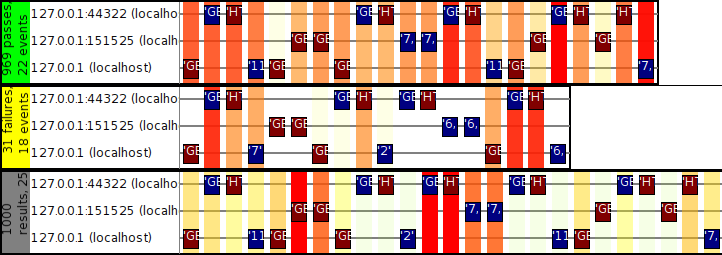
\includegraphics[width=\linewidth]{hue-mapping}
  \caption{Hue Mapping For Events}
  \label{fig:hue-mapping}
\end{figure}

\section{Reordering Access to Network Resources}
\label{sec:reord-access-shar}

In our prototype we support re-scheduling network access in the live
system. Parallel network events inherently cause races, the network
transport may transmit messages at different speeds and the operating
system may forward messages to user space applications as it sees
fit. To reorder access to network resources, the network events have
to arrive at the application in order, so network events have to be
re-ordered in a layer between the application and the hardware.

We decided to re-order events in the language, using the same
mechanism as for tracing. We use ContextS to define a scheduler layer
between applications and the KomHttpServer framework and the Squeak
standard library (\cf{\autoref{fig:structure}}). This scheduler layer
is only active if a schedule was requested.

\subsection{Constraints on the Networked Systems}
\label{sec:constr-netw-syst}

Our design is supposed to work for local systems on the developer
machine, in test environments and the live system. However, because we
only record communication partners and the partial ordering of events,
in practice, there are various constraints on those systems. First,
hey have to be deterministic in their communication, which means if we
send them messages in the right order, they return valid responses in
right order. This means have to be able to control the order in which
messages are received. However, with systems that employ load
balancing, multi-threading and event loops which are designed to
handle multiple requests in parallel we cannot be sure that for
multiple requests the responses are generated in order. This means we
have to control the send order, too.

\subsection{Entry Points}
\label{sec:entry-points}

According to the design, there are two types of entry points which we
need to control to enable re-scheduling, both for sending and
receiving. We only deal with \ac{http} requests and, because we use
the same context-oriented mechanism as for the tracer, we only had to
create a layer to wrap the same three methods as for the tracer. Our
scheduler layer is always active and the wrapper methods check whether
a schedule was requested. This check simply uses a globally available
singleton object and checks whether it contains a valid schedule. If
not, the scheduler methods do nothing and simply proceed.

\subsection{Scheduling Execution}
\label{sec:scheduling-execution}

Our implementation follows the design shown in
\autoref{fig:reorder-sched}. The framework we used to implement our
example application uses threads to handle multiple connections, so
for simplicity, we have only implemented the threading scheduler using
semaphore queues.

To schedule an execution, the trace that is used as basis for the
execution is copied and transformed into a list of schedulable
events. All of these events contain the identifiers for the original
communication partners, the id of the event and a semaphore in the
\emph{waiting} state. This list is then attached to the globally
accessible singleton object and the first semaphore is
signaled. Finally, the diagnosis script is started to provide the
required events.

\paragraph{Receive}
\label{sec:receive}

The KomHttpServer uses a blocking \emph{accept} call on a socket
object to wait for incoming requests, which the \ac{vm} translates
into the \emph{accept} system call. When that call returns, the
operating system socket has data available. The KomHttpServer
framework then spawns a new thread that creates an
\emph{HttpRequest} object from the received data and passes this
into the application.

Before it passes from framework to application code it has to go
through our scheduler. The scheduler uses an atomic operation to find
the appropriate event in the schedule for this request, attach the
request object onto it, and return the event object from the
schedule. It then calls \emph{wait} on the event object's
semaphore. If the semaphore was already signaled this call returns
directly, otherwise this thread blocks until the semaphore is
signaled.

When the \emph{wait} call to the semaphore eventually returns, the
semaphore for the following event is signaled and the request object
is passed back into the framework, from which it passes on into
application level code.

\paragraph{Send}
\label{sec:send}

Sending of data works similarly. The application manufactures an
\emph{HttpResponse} object and returns it to the framework. The
framework the calls the \emph{writeOn:} method with the socket object
to serialize the response onto the socket stream. We wrap this method
and use the atomic find, set, and return operation on the schedule to
find the scheduled event corresponding to this response, and then wait
on the semaphore. When semaphore is signaled, we proceed to the base
method which writes the response to the network.

The fact that we have only implemented the semaphore list for our
scheduler means that means it is currently limited by the maximum
amount of threads available to the framework for handling multiple
connections. Because each thread blocks if the event cannot be
released directly there may be situations in which so many threads are
blocked that the framework cannot create any more threads for incoming
requests, at which point the server will deadlock. We circumvent this
problem in our implementation by having the semaphore wait time out
after a configurable amount of time, after which point the
re-scheduling deviates from the desired schedule.

\subsection{Probable Replay}
\label{sec:probable-replay}

A goal for a scheduler following our design is to enable consistent
replay. Our design only works for well-behaved clients and stable
networks, constraints that cannot always be guaranteed in a real
environment. However, these constraints may often be met, even if not
all the time. A practical re-scheduler may not always work, but it
raises the probability that a specific schedule will be reproduced,
and it will reproduce the schedule if the circumstances permit. If the
network is sufficiently disturbed, either because of misbehaving
clients or connection problems, the scheduler deals with it by
deviating from the desired schedule.

As mentioned above, our implementation uses timeouts to make sure that
the distributed system does not lock up, but timeouts include the
potential for releasing events too early and thus deviate from the
desired schedule, causing a re-execution inconsistent with the
original trace. Our implementation also continually checks for
disturbances defined in
\autoref{sec:required-heuristics}---unscheduled events, schedule
disruptions by misbehaving clients---and we have implemented
configuration settings that determine how we deal with them. These
settings currently allow developers to choose to drop unscheduled
events, or pass them through without waiting for a semaphore. Our
implementation additionally uses simple printf logging to communicate
to the developers how it is reshaping the network schedule, i.e. which
events have been encountered, which are being waited for, and which
disturbances were encountered and how were they dealt with.

\section{Connecting Network and Object Communication}
\label{sec:conn-netw-object}

Adequate tools are essential for efficient debugging. Previous
approaches at efficient replay for the most part focus on recording
and replaying correctly and efficiently, but use existing debuggers
like \emph{GDB} for interactions with the program state, and separate
tools to review the captured network data. Other approaches, like
\emph{Causeway}, focus on the tools.

We think that the debugging tool should be integrated, allowing the
user to inspect both object and network communication in one view, as
they are in Causeway. However, efficient replay is required for those
tools to be practical, so a recording and replay mechanism like our
scheduler has to be integrated into the tool.

Our prototype extends the call tree view, called \emph{Path Finder},
which is part of the Path Tools suite. Our tool, inspired by Causeway,
shows network communication and the call tree for one server in a
single window. These views should be synchronized, so if a user opens
a method, the closest network event should highlighted. Inversely,
clicking on a network event should open the call tree on the method
that is closest to the network event. If the network event was sent or
received on the server to which the call tree belongs, it should show
the method responsible for the event.

For this prototype, we have only implemented moving from the network
to the code view, not vice-versa. If a user clicks on a network event,
the scheduler is instructed to record the stack at the time of the
network event and the test case is re-executed. We then search for a
method on the stack that is part of our call tree, and open that
method for inspection. In \autoref{fig:pathfinder} we show the result
of clicking on the third network event~\textcircled{1}. In the lower
part of the window, the call tree is expanded to the method which sent
the event.

\begin{figure}
  \centering
  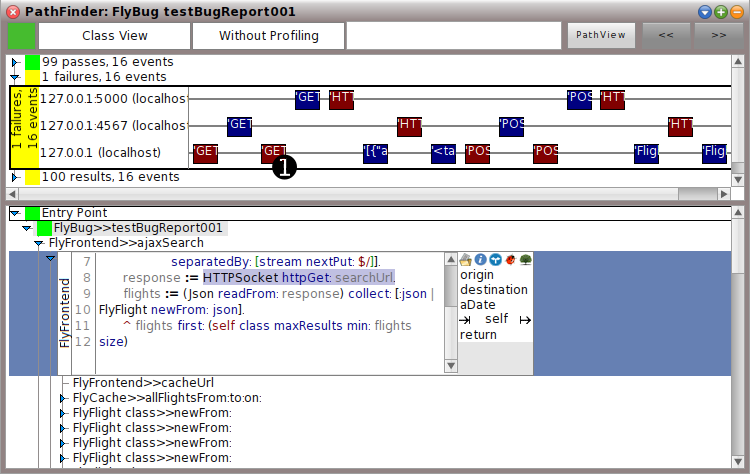
\includegraphics[width=0.9\linewidth]{pathfinder}
  \caption{The Path Finder Network Extension}
  \label{fig:pathfinder}
\end{figure}

A full implementation should support full synchronization between the
two views. We have also not implemented additional queries of the
program state. A fully implemented tool should support queries of
single variable values, method arguments and other program state in
the scheduler, to allow further inspection of the program state.

%%% Local Variables: 
%%% mode: latex
%%% TeX-master: "thesis"
%%% End: 
